%File: formatting-instruction.tex
\documentclass[letterpaper]{article}
% AAAI format packages
\usepackage{aaai}
\usepackage{times}
\usepackage{helvet}
\usepackage{courier}
% Additional packages
\usepackage{amsmath}
\usepackage{amssymb}
\usepackage{amsthm}
\usepackage{algorithm}
\usepackage{algorithmic}
\usepackage{graphicx}
\usepackage{comment}
\newtheorem{thm}{Theorem}
\newtheorem{defn}{Definition}
% END Additional packages
\frenchspacing
\setlength{\pdfpagewidth}{8.5in}
\setlength{\pdfpageheight}{11in}
\pdfinfo{
/Title (Experience-Biased Symbolic Planning)
/Author (Aram Ebtekar, Mike Phillips, Sven Koenig, Maxim Likhachev)
/Keywords (symbolic planning, E-Graph, experience-biased, weighted A* search, STRIPS, HSP)
}
\setcounter{secnumdepth}{0}  
 \begin{document}
% The file aaai.sty is the style file for AAAI Press 
% proceedings, working notes, and technical reports.
%
\title{Experience-Biased Symbolic Planning}
\author{Aram Ebtekar$^\dagger$ \and Mike Phillips$^\dagger$ \and Sven Koenig\thanks{University of Southern California, Los Angeles, CA 90089} \and Maxim Likhachev% <-this % stops a space
\thanks{Carnegie Mellon University, Pittsburgh, PA 15217}% <-this % stops a space
%
}
\author{SoCS 2014 Submission 2}% anonymizer
\maketitle
\begin{abstract}
\begin{quote}
Weighted A* search is the foundation for state-of-the-art domain-independent symbolic planners.
An important open challenge for these planners is to utilize experience with similar planning problems to speed up subsequent planning episodes.
Experience graphs have recently shown promise as a technique for plan reuse in the context of weighted A* searches in robotics, by biasing them towards a subgraph of the search space, typically chosen to consist of the edges used in previous plans.
In this paper, we demonstrate how to augment symbolic planners with
experience graphs, using the HSP2 planner as a representative
example.
The resulting planners are able to trade off seamlessly
between plan quality and runtime and thus have advantages over past
plan-reuse techniques, such as planning by analogy.
We demonstrate experimentally that on many symbolic domains, our approach reduces the number of nodes that the HSP2 planner needs to consider by a factor of 2 or more while achieving about the same plan quality.
\end{quote}
\end{abstract}

\section{Introduction}

\begin{comment}
Planning entails finding action sequences that achieve a goal state.
In order to apply the language of graph theory, states are often thought of as nodes connected by action transitions.
A \textbf{plan} is a path from the start state to one of many goal states.
Despite the existence of classic polynomial-time search techniques, such as Dijkstra's algorithm, planning remains the crux of many difficult problems in AI.

The reason usually is that the graphs involved are very large; indeed, too large for explicit storage.
In motion planning, the state space may be a continuous geometric set whose desired discretization is very fine.
In symbolic planning, a planning language such as STRIPS, SAS+, ADL or PDDL [CITE] is chosen to give a compressed symbolic representation.

The graph is exponentially larger than its encoding so, in both cases, states are generated only as needed.
The symbolic representation sometimes encodes exploitable structure.
In order to create a domain-independent solver for a language such as STRIPS, we need to automatically extract and interpret structural information about the problem. 

In forward weighted A* search, a frontier of nodes expands from the start until it hits a goal, at which point a solution is found.
Rather than blindly searching the entire exponential-sized space, A* tries to focus toward the goal by expanding nodes which seem likely to lie on a short solution path.
The minimum length of a solution passing through a given frontier node is the sum of distances from the start to this node, and from this node to a goal.
The better we estimate these, the sooner we'll reach a solution.

Since A* expands in a fairly conservative fashion from the start state onward, the start-to-frontier estimates are very well-approximated by construction of a valid path.
Thus, the principal issue is the derivation of frontier-to-goal estimates.
Given exact distances, it would be a simple matter to trace a valid path from the start, taking optimal successors at each step, until a goal is reached.
In practice, we are forced to use estimates, which sometimes mislead us into local optima, wasting time on dead-end nodes.

These distance approximations are called \textbf{heuristics}, and we use them in hopes of finding good plans more efficiently.
Algorithms such as A* are designed to find solutions quickly whenever the heuristic is of reasonable quality.
If we hope to take subexponential time, we can only afford to examine a vanishing fraction of the states, and it is only for these that we compute the heuristic.
If the heuristic is good, we hope not to have to visit (i.e. generate) too many states.
Hence, there is a tradeoff between spending more time to compute a more accurate heuristic, vs evaluating a weaker heuristic quickly but at many more states.

In practice, even using state-of-the-art methods to generate heuristics on isolated planning instances, STRIPS problems can be very difficult to solve without expert domain knowledge.
Even humans have difficulty when faced with an unfamiliar kind of puzzle, though we get better with experience.
Thus, one might hope that a planning agent would similarly learn to generalize solutions from past planning experiences to related new instances.
\end{comment}

Modern state-of-the-art symbolic planners tend to rely on weighted A* search as their core algorithm.
In forward weighted A* search, a frontier of nodes expands from the start until it hits a goal, at which point a solution is found.
The performance of weighted A* depends heavily on its \textit{heuristics}, cheaply computable approximations of the remaining distance from a given node to the goal. Heuristics focus the efforts of weighted A* toward the goal and can greatly impact the runtime of the search.
Consequently, much research has been devoted to developing new heuristic functions and different techniques for combining multiple heuristic functions together, all with the aim of providing more effective guidance to the weighted A* search.

However, even with good heuristic functions, many symbolic planning problems can be very difficult to solve.
A state-of-the-art domain-independent planner, or even a human faced with an unfamiliar kind of problem, might have great difficulty in solving it.
After having solved several instances of a problem, humans tend to utilize their experience and learn how to solve similar problems quickly.
Similarly, it is beneficial to develop planning algorithms that can learn to solve repeated planning problems faster over time.

In robotics, Experience Graphs (E-Graphs) have recently been introduced as a means of accelerating motion planning from experience~\cite{phillips2012graphs}.
Based on previously computed plans (a.k.a. experiences), this methods computes an E-Graph that models the high-level connectivity of the free space in motion planning tasks.
The intuition is to remember previously generated paths so that, when a new start and goals are queried, a new path can be quickly generated by reusing subpaths from the E-Graph.
A variant of weighted A* is employed which biases its focus toward the E-Graph.
While this work demonstrates promising results in robot motion planning, E-Graphs have never before been applied to symbolic domain representations such as the STRIPS language.

Our present contribution is to investigate the use of E-Graphs in STRIPS domains. In particular, we take the HSP2 planner~\cite{bonet2001planning} as a representative of the class of modern symbolic planners that are based on weighted A*, and augment its heuristic with a bias toward its E-Graph. After presenting the related works, we begin by describing the STRIPS language and the original HSP heuristic. In the following section, we formally introduce E-Graphs in technical detail. Then we combine the two approaches, resulting in the new Experience-Biased HSP planner. We present the algorithm and discuss its theoretical properties. This is followed by experiments showing promise for the application of E-Graphs to symbolic problem solving. Finally, we conclude with some thoughts on extensions worth investigating.

\section{Related Works}

Classically, case-based reasoning methods 
such as PRIAR~\cite{Kamb:92}, SPA~\cite{Hank:95}, MRL~\cite{Koeh:94}, and NoLimit~\cite{mljournal}
have been used to recall 
previous plans that appear similar to the current problem, and 
then adapt them to meet the new specifications.
Compared to these methods, our work reuses prior experience in
the context of modern weighted A*-based methods for symbolic planning. We also provide
a bound on the suboptimality of the solution.

Recently, there has been work on incorporating prior knowledge 
into modern planners (based on weighted A* and powerful heuristics).
For instance, GPG~\cite{Gere:00} uses planning graphs to adapt a prior path to the 
new scenario by searching locally within windows around plan 
inconsistencies. To guarantee completeness, the windows can grow 
if solutions are not found until they constrain the whole plan.
In this work~\cite{DBLP:conf/iccbr/RosaOB07}, case-based reasoning is used to choose the 
order of state evaluations of EHC (enforced hill-climbing), which 
is a component in modern planners such as FF. 

OAKplan~\cite{Serina:2010:KFC:1860143.1860472} is a recent 
case-based reasoning method which converts 
planning instances into a compact graph representation, and 
then uses recent kernel methods for matching labeled graphs to select
a similar case to the problem at hand. The selected case is then 
adapted using LPG-ADAPT~\cite{Fox06planstability}. LPG-ADAPT is a replanning method
that encourages \textit{plan stability}: it tries to make 
sure that the new plan is as similar to the previous plan as possible. 
The method also uses a modern heuristic search approach. While E-Graphs too can encourage stability by reusing old plans, our primary purpose is efficient planning with cost suboptimality bounds, rather than stability.

ERRT-PLAN~\cite{workshop-icaps12-errtplan} presents a very different 
approach to reuse in planning. 
Similar to E-Graphs, ERRT has its roots in motion planning~\cite{Bruce:2002}.
ERRT-PLAN applies this sampling-based motion planner that leverages 
reuse to symbolic planning. The planner randomly chooses to extend 
the search tree toward the goal, toward subgoals from previous 
plans, or to reuse an action from a previous plan. 
The extension operations are based on modern heuristic search
planners.
The stochastic nature of the direction the search progresses toward
allows it to overcome local minima caused by misleading heuristics.

The primary difference between our approach and previous works 
is that we plan with prior experience in a way that comes with provable
bounds on the suboptimality of the solution. The use of E-Graphs also
allows us to formulate this in such a way that the user has control over
this suboptimality bound with an intuitive parameter that trades
reuse (speed) for solution quality.

The HSP2~\cite{bonet2001planning} planner uses the heuristic pioneered by HSP, but replaces greedy hill-climbing with weighted A* search.
We test our approach on HSP2 because the latter is straightforward to describe, and because it is representative of the core techniques that are common to many state-of-the-art domain-independent symbolic planners.
Some newer additions to the field include the causal graph heuristic of the Fast Downward planner~\cite{helmert2006fast} and the landmark heuristic of the LAMA planner~\cite{richter2010lama}. Our approach is orthogonal to these developments and can, in principle, be adapted to work with any search heuristic.

\section{STRIPS Language}

A STRIPS problem is a tuple $P = \langle A,O,I,G\rangle$ consisting of an atom set $A$, operator set $O$, initial state $I \subseteq A$ and goal condition $G \subseteq A$.
Each operator $op\in O$ is defined by its cost, preconditions, add effects and delete effects: $Cost(op) \in \mathbb{R}^+$ and $Prec(op),Add(op),Del(op) \subseteq A$.

The problem $P$ defines a directed state graph $(V,c)$ where $V$ is the power set of $A$ (i.e. states $S\in V$ correspond to collections of atoms), and the edge costs are
\begin{eqnarray*} c(S,S') = \min\{Cost(op) \mid S\supseteq Prec(op)\text{ and}
\\S' = \left(S \setminus Del(op)\right) \cup Add(op)\} \end{eqnarray*}
%consists of states transitions $(u,v)$ for which there exists an operator $op\in O$ with $u\in Prec(op)$ and $v = u - Del(op) \cup Add(op)$; the weight of this edge is the minimum cost of such an $op$.
By default, $c(S,S') = \infty$ when there is no operator directly transitioning from $S$ to $S'$.
Given a STRIPS problem $P$, we seek a low-cost path from the initial state $I\in V$ to any of the goal states $S\in V$ such that $S \supseteq G$. In this paper, we are particularly concerned with sequences of problems in which $A$ and $O$ are fixed, but various pairs $\langle I,G\rangle$ are queried.

\section{HSP Heuristic}

Many of today's state-of-the-art domain-independent STRIPS planners are based on the HSP2 planner~\cite{bonet2001planning}, which we now describe.
It's common to compute heuristics by solving an easier, relaxed version of the original problem. In STRIPS, one might ignore the delete lists of operations.
Since having more atoms makes preconditions and the goal condition more likely to hold, this can only make the problem easier, so the heuristic derived from relaxation never overestimates the true cost.

However, even the relaxed STRIPS planning problem includes set-cover as a special case, making it NP-hard.
Intuitively, we see that the relaxed search space remains exponential in size.
To reduce it, HSP2 decouples the atoms, instead estimating the cost of achieving each individual atom.

Let's say we want a heuristic estimate of the distance from state $S$ to a goal that contains $G$. HSP2 estimates the cost to achieve an atom $a\in A$ from $S$ by $g_S(a) = $
\[\begin{cases} 0  &\mbox{if } a \in S
\\ \min_{op\mid a\in Add(op)} \left(g_S(Prec(op)) + Cost(op)\right)  &\mbox{if } a \notin S \end{cases}\]

The HSP heuristic (also used in HSP2) is then defined by
\[h^{HSP}(S) = g_S(G),\]
the estimated cost of achieving all atoms in $G$. Note that $g_S(\cdot)$ is evaluated on certain atom sets, namely $Prec(op)$ and $G$.
To keep the computations feasible, define $g_S(P) = \max_{p\in P} g_S(p)$ for atom sets $P$.
The resulting HSP-max heuristic is an underestimate; indeed, it satisfies a stronger property called consistency.

\begin{defn} For $\epsilon\ge 1$, a heuristic $h$ is called \textbf{$\epsilon$-consistent} iff $h(S) = 0$ when $S$ is a goal and $h(S) \le \epsilon c(S,S') + h(S')$ for all $S,S'\in V$. $h$ is \textbf{consistent} iff it is $1$-consistent. \end{defn}
\begin{thm} Given an $\epsilon$-consistent heuristic, A* without reexpansions is guaranteed to find a path costing no more than $\epsilon$ times the optimal path cost~\cite{LikGorThr-ara}. \end{thm}

If the atoms were completely independent, a more accurate estimate would be $g_S(P) = \sum_{p\in P} g_S(p)$.
Despite its inconsistency in general, the latter HSP-plus heuristic is often useful in practice, as it uses more state information: it decreases if progress is made towards \textit{any} goal atom, instead of just the most distant goal.

From a computational perspective, the HSP heuristic must compute $g_S(a)$ for all $a\in A$ whenever a new state $S$ is generated.
This can be done by dynamic programming, iterating the recursive formula to a fixpoint in Bellman-Ford-like fashion.
Pseudocode is listed in Algorithm \ref{alg:ComputeG}.

\begin{algorithm}
\caption{ComputeG($S$)}
\label{alg:ComputeG}
\begin{algorithmic}
\FORALL{$a \in A$}
\IF{$a \in S$}
\STATE $g_S(a) \leftarrow 0$
\ELSE
\STATE $g_S(a) \leftarrow \infty$
\ENDIF
\ENDFOR
\REPEAT
\FORALL{$op \in O$}
\STATE $cost\_estimate \leftarrow g_S(Prec(op)) + Cost(op)$
\FORALL{$a \in Add(op)$}
\STATE $g_S(a) \leftarrow \min \left(g_S(a),~cost\_estimate\right)$
\ENDFOR
\ENDFOR
\UNTIL{no further change in $g_S$-values}
\end{algorithmic}
\end{algorithm}

\section{Experience Graphs}

E-Graphs can improve total search time over a series of related queries on the same graph.
Formally, an E-Graph is a subgraph of the state space.
It is updated between queries, typically by adding the solution path from the previous search query.

Suppose we have a consistent heuristic $h(S,S')$ for the distance between arbitrary pairs of states.
That is, $h$ obeys the triangle inequality, is never dominated by an edge cost, and $h(S,S) = 0$ for all $S\in V$.

Planning with E-Graphs is simply a matter of running weighted A* search with the \textbf{E-graph heuristic} $h^E$, derived from $h$.
$h^E$ biases the search to follow E-Graph edges instead of $h$ by penalizing the latter by an inflation factor $\epsilon^E > 1$.
To be precise, define

\[h^E(S_0) = \min_{N,S_N,\pi} \sum_{i=1}^N \min \left(\epsilon^E h(S_{i-1},S_i),c^E(S_{i-1},S_i)\right)\]
with the minimization taking place over all goal states $S_N$ and all paths $\pi = \langle S_0,S_1,...,S_N \rangle$ of arbitrary length.

$c^E$ encodes E-Graph edge costs, or $\infty$ if the corresponding edge is not a part of the E-Graph.

In the limit as $\epsilon^E \rightarrow 1$, E-Graph edges offer no advantage because $h(S_{i-1},S_i) \le c^E(S_{i-1},S_i)$. Hence, using the triangle inequality to coalesce the sum,
\[h^E(S_0) = \min_{N,S_N,\pi} \sum_{i=1}^N h(S_{i-1},S_i) = \min_{S_N} h(S_0,S_N)\]

Conversely, as $\epsilon^E \rightarrow\infty$, the inflated terms dominate. Hence, the minimizing path becomes one which incurs the least estimated cost outside the E-Graph. In particular, $h^E$ has the following property:

\textit{For sufficiently large $\epsilon^E$, once the A* frontier touches an E-Graph component which includes a goal state, no node outside the E-Graph will ever again need to be expanded.}

This means, for instance, that if the E-Graph already contains a path from the start to a goal, then A*, guided by $h^E$ with large bias parameter $\epsilon^E$, will never leave the E-Graph.
If the E-Graph is small, a solution would promptly be discovered.
In this manner, little work is needed to solve previously encountered subproblems.

We cannot afford to compute $h^E$ according to its literal definition, as there are far too many paths to consider.
Fortunately, there exists a practical means of computing it. By the triangle inequality, any consecutive pair of $h(S_{i-1},S_i)$ terms can be merged into one.
Thus, we lose no generality in restricting $S_i$ to lie on the E-Graph for $0 < i < N$.
The heuristic computation can focus on the E-Graph, using $h(S_{i-1},S_i)$ to estimate the cost of leaving the E-Graph at $S_{i-1}$ before reentering it at $S_i$.

Let $V^E$ be the union of the goal states and the E-Graph's vertices.
In addition to following E-Graph edges, we imagine it's possible to ``jump" from any $S\in V^E$ to any $S'\in V^E$ at cost $\epsilon^E h(S,S')$.
That is, let
\[c'(S,S') = \min\left(c^E(S,S'),~\epsilon^E h(S,S')\right)\]


In a preprocessing stage before the main search, we apply Dijkstra's algorithm once in reverse with the costs $c'$ to compute the estimated distance-to-goal $h^E(S)$ from every $S\in V^E$. Ignoring the computation of $h$ (presently considered as a blackbox), this preprocessing takes $O(|V^E|^2)$ time, which is insignificant for small E-Graphs and goal sets.

Later, when A* generates $S \notin V^E$, we see that we have already precomputed costs of paths consisting of all but the first edge of the minimizing path $\pi$ in the definition of $h^E(S)$. Thus, we derive the mathematically equivalent but much cheaper computation
\[h^E(S) = \min_{S'\in V^E} \left(\epsilon^E h(S,S') + h^E(S')\right)\]

\begin{thm} If the base heuristic $h$ is consistent, then $h^E$ is $\epsilon^E$-consistent~\cite{phillips2012graphs}.\end{thm}

\begin{figure}
	\begin{center}
	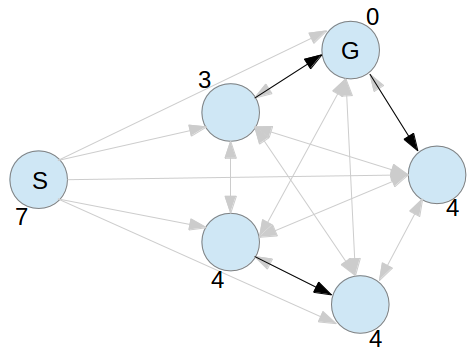
\includegraphics[scale=0.5]{Pentagon.png}
	\end{center}
	\caption{An example E-Graph with three edges, and corresponding $h^E$-values. $S$ is not on the E-graph.}
	\label{fig:example}
\end{figure}

Figure \ref{fig:example} illustrates the idea. Suppose the dark edges have cost 3 and make up the E-Graph. Off-E-Graph edges are not shown, as they are only referenced indirectly via $h$; instead, light edges represent the jump estimates $h(S_i,S_j) = 2$ (with one exception: $h(S,G) = 5$), which we inflate by a factor $\epsilon^E=2$ to make 4 (or 10, respectively). Dijkstra's algorithm follows dark and light edges backward to compute the $h^E$ values shown alongside each node.

$G$ is on the E-Graph, though this need not be the case in general. $V^E$ is the pentagon on the right, and its $h^E$ values are precomputed before the search. For $S\notin V^E$, $h^E(S)$ is computed only when A* generates $S$.

\section{Experience-Biased HSP}

We now combine the ideas from HSP2 and E-Graphs to construct a domain-independent STRIPS planner which learns from experience. In STRIPS, a consistent heuristic $h(S,S')$ is given by the HSP-max estimate $g_S(S')$. We can compute $g_S(S')$ for all $S,S'\in V^E$ in precisely $|V^E|$ runs of Algorithm \ref{alg:ComputeG}: each run provides us with $|V^E|$ of these values, yielding $|V^E|^2$ values in total.

As before, Dijkstra's algorithm inflates and combines these estimates with the E-Graph edges to derive $h^E(S)$ for all $S\in V^E$. Note that in STRIPS, $V^E$ need not include every goal state: the minimal goal $G$ suffices as it's always the easiest to reach in the heuristic relaxation.

Upon encountering a new state $S\notin V^E$, we run Algorithm \ref{alg:ComputeG} again to compute $g_S(a)$ for all atoms $a\in A$. Then it's a simple matter to compute the E-Graph heuristic by

\[h^E(S) = \min_{S'\in V^E} \left( \epsilon^E g_S(S') + h^E(S') \right)\]

We remark that, when E-Graphs are involved, the values $g_S(S')$ on the right-hand side range over a variety of different states $S'$. Compare this to the formula for $h^{HSP}$, which uses only $g_S(G)$. HSP2 would still compute all the $g_S$-values despite using them only once, so here we get to consult the E-Graph essentially for free. The only additional work is the minimization over $S'\in V^E$, which takes O($|V^E||A|$) time. A pseudocode implementation is listed in Algorithm \ref{alg:Search}. The parameter $\epsilon^E$ controls bias toward the E-Graph, while the weight $\epsilon$ provides a uniform goal-directed bias.

\begin{algorithm}
\caption{Search()}
\label{alg:Search}
\begin{algorithmic}
\FORALL{$S \in V^E$}
\STATE ComputeG($S$)
\FORALL{$S' \in V^E$}
\STATE $c'(S,S') \leftarrow \min\left(c^E(S,S'),~\epsilon^E g_S(S')\right)$
\ENDFOR
\ENDFOR
\STATE Compute $h^E$ on $V^E$ by reverse Dijkstra from $G$ with $c'$.
\STATE Run A* on the full graph from $I$ with heuristic $\epsilon h^E$:
\FOR{$S \notin V^E$ when generated by A*}
\STATE ComputeG($S$)
\STATE $h^E(S) \leftarrow \min_{S'\in V^E} \left( \epsilon^E g_S(S') + h^E(S') \right)$
\ENDFOR
\IF{A* successfully found a path to some goal state $S \supseteq G$}
\STATE Add all edges of the solution path to the E-Graph.
\RETURN solution path
\ELSE
\RETURN failure
\ENDIF
\end{algorithmic}
\end{algorithm}

ComputeG($S$) implements the dynamic programming computation of $g_S$-values.
Each iteration of the outermost loop permanently fixes at least one $g_S(a)$ value, so it does at most $|A|+1$ iterations.
Multiplying nested loop iterations together and dropping cardinality signs for brevity, a conservative runtime bound on Algorithm \ref{alg:ComputeG} is $O(\mathbf{A^2O})$.
Therefore, it costs $O(\mathbf{A^2O + V^EA})$ time to generate each state.

The preprocessing cost is $O(\mathbf{V^EA^2O + (V^E)^2A})$, asymptotically equivalent to preemptively generating every state in $V^E$.
In fact, most of the preprocessing requires no knowledge of $G$, so it can be done in advance of the new planning query. Once the query $\langle I,G\rangle$ is given, the remaining work consists of completing the $c'(S,G)$ computations from $g_S(a),a\in G$, and then running Dijkstra's algorithm from $G$. This costs only $O(\mathbf{V^E(A + V^E)})$ time.

For comparison, standard HSP2 without E-Graphs takes $O(\mathbf{A^2O})$ time (with essentially the same constant factors) to generate each state, and does not incur the cost of generating a state unless the A* frontier encounters it.
When HSP2 is augmented with small E-Graphs, the same asymptotic bound continues to hold, provided that the number of E-Graph vertices is limited to $O(\mathbf{AO})$. Furthermore, we retain completeness and the ability to configure suboptimality bounds by adjusting the bias parameters:

\begin{thm}
If there exists a path from initial state $I$ to a goal state $S\supseteq G$, the experience-biased HSP-max search algorithm finds a path which is at most $\epsilon\epsilon^E$-suboptimal.
\end{thm}

This follows directly from Theorems 1 and 2, since the weighted heuristic $\epsilon h^E$ is $\epsilon \epsilon^E$-consistent.
However, E-Graphs make no guarantee of improving the search time. Indeed, biasing toward bad regions could trap the planner inside large local optima.
Potential gains depend entirely on choosing a good small set of edges to form our E-Graph.
In our experiments, we simply keep the previous solution path; different choices remain a topic for future investigations.

\section{Experiments}

We augmented the original HSP2 planner code~\cite{bonet2001planning} with E-Graphs.
Since HSP-plus performs better in practice than HSP-max, we take the former heuristic as our baseline.
The purpose is to measure how E-Graphs affect the number of states generated by the planner in various STRIPS domains.
We prepared two experiments, each presenting scenarios in which we hope for the planner to learn from experience.
The STRIPS problems are taken from the HSP2 test suite; we note that every operator in these problems has cost 1.

\subsection{Experiment 1: Reusing Fragmented Experiences}

In this experiment, we solve several hundred problem instances spanning 18 symbolic domains.
For each problem, we first plan without experiences, using the HSP-plus heuristic in an A* search with weight $\epsilon=5$.
This search acts as our scientific \textbf{control}.
If the control fails to find a solution within 5 seconds (on an Intel Core i7-2600), we discard the problem instance.
Otherwise, we record the plan cost and the number of states that were generated during the search.
Thus, we end up recording data for 321 problem instances.

For each of these, we run 3 additional searches using E-Graphs, setting $\epsilon^E=5$ but reducing $\epsilon$ to 1, thus maintaining the same theoretical suboptimality bound as planning with no E-Graph weighted by $\epsilon=5$.
(Note that although $\epsilon = 1$, some inflation is implicit in the use of HSP-plus.
HSP-plus may overestimate by a factor equal to the number of atoms in the goal in the worst case, but only if the atoms are extremely highly coupled.)

The E-Graph consists of 20\%, 50\% or 80\% of the edges selected at random from the control's solution path, over the 3 respective searches. For each of these, we again record the solution cost and number of nodes generated, and compare these figures against the control.
We define \textbf{speedup} as the ratio of the number of nodes generated in the control to the number generated in the E-Graph search.
Likewise, we define the \textbf{cost improvement} as the ratio of solution cost in the control to cost in the E-Graph search.

Results are summarized in Table \ref{tab:percent}.
To estimate the typical range of speedups, we present the 25th and 75th percentile speedups among the instances of each domain.
The full data from Experiment 1 is plotted in Figures \ref{fig:s_20_0} to \ref{fig:s_80_0}.
We see that, while performance is virtually unaffected in some domains, it's never substantially worsened and, in certain domains, the experience helps greatly.
For example, results are highly encouraging in the Blocks domain.
Furthermore, Figure \ref{fig:c_50_0} shows that the solution quality remains competitive; indeed, we see that when E-Graphs are employed, the path cost is slightly reduced on average.

Note that using 100\%, or perhaps even 80\%, of the E-Graph would seem to trivially grant us the solution, as we could simply follow the remembered path depth-first.
In practice, since we fixed the bias parameter to $\epsilon^E=5$ rather than raising it to an extremely large value, the search expands a fair number of states even if we remember most or all of the path.
This is necessary to ensure the suboptimality bound, as the planner does not know whether the E-Graph can be ``trusted" to yield an efficient path.
E-graphs are used as suggestions, not as a trusted form of knowledge; the planner remains responsible for proving suboptimality.

\begin{figure}
	\centering
	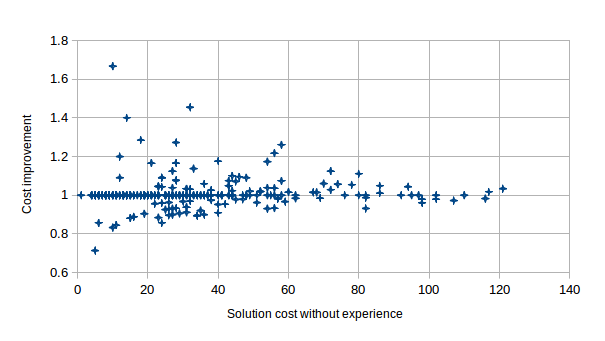
\includegraphics[scale=0.5]{Cost_50_0.png}
	\caption{Relative plan costs using 50\% of the control experience, displaced 0 steps from the control query.}
	 \label{fig:c_50_0}
\end{figure}

\begin{table}
	\centering
	\resizebox{\columnwidth}{!}{%
	    \begin{tabular}{| r | c | c | c | c |}
	    \hline
	    Domain & Count & 20\% exp & 50\% exp & 80\% exp
	    \\ \hline
	    blocks & 35 & 1.08-1.82 & 1.37-3.73 & 1.90-5.84
	    \\ 
	    driverlog & 14 & 1.00-1.49 & 1.11-1.58 & 1.15-1.60
	    \\ 
	    elevators & 30 & 1.00-1.62 & 1.00-2.84 & 1.04-3.19
	    \\ 
	    freecell & 34 & 1.00-1.06 & 1.00-1.12 & 1.00-1.08
	    \\ 
	    grid & 2 & 1.07-1.18 & 2.16-3.57 & 2.22-3.75
	    \\ 
	    logistics00 & 28 & 0.91-1.04 & 0.98-1.13 & 1.03-1.19
	    \\ 
	    logistics98 & 5 & 0.95-1.01 & 1.09-1.62 & 1.24-3.00
	    \\ 
	    mprime & 19 & 1.00-1.00 & 1.00-1.07 & 1.00-2.46
	    \\ 
	    pegsolitaire & 29 & 1.00-3.57 & 1.13-4.49 & 1.68-6.63
	    \\ 
	    pipesworld-notankage & 15 & 1.00-3.27 & 1.00-7.07 & 1.00-9.95
	    \\ 
	    pipesworld-tankage & 8 & 1.00-1.00 & 1.00-1.02 & 1.00-1.45
	    \\ 
	    rovers & 13 & 0.97-1.23 & 1.23-7.09 & 1.23-7.17
	    \\ 
	    satellite & 16 & 0.99-1.00 & 1.00-1.26 & 1.00-1.26
	    \\ 
	    scananalyzer & 16 & 1.00-1.15 & 0.93-1.20 & 1.00-1.36
	    \\ 
	    sokoban & 11 & 1.12-2.10 & 1.32-3.02 & 1.56-7.80
	    \\ 
	    tpp & 10 & 1.00-1.00 & 1.00-1.23 & 1.00-2.31
	    \\ 
	    transport & 23 & 1.00-1.14 & 1.09-1.86 & 1.19-1.89
	    \\ 
	    zenotravel & 13 & 1.02-1.15 & 1.08-1.44 & 1.14-1.58
	    \\ \hline
	    TOTAL & 321 & 1.00-1.29 & 1.00-1.91 & 1.02-2.68
	    \\ \hline
	    \end{tabular}%
	}
	\caption{Experiment 1 speedup statistics, summarized in the form (1st quartile)-(3rd quartile).}
	 \label{tab:percent}
\end{table}

\subsection{Experiment 2: Reusing Nearby Experiences}

The previous experiment tested our ability to complete partial plans that are fragmented by gaps; however, the experimental searches solved identically the same problems as the control used to generate the E-Graph.
Now, we try changing the start and goal states by moving each of them a small distance within the state space. 
In this manner, we test how well E-Graphs enable the planner to generalize to nearby but non-identical queries.

We narrow our focus to 13 domains, and take from each of them the same set of instances as in Experiment 1, yielding 218 problem instances in all.
This time, we save 100\% of the solution path found by the problem's corresponding control from Experiment 1.
Then, for each problem, we form 3 modified problems where the start and goal are each displaced by 5, 20 or 50 steps, respectively, of random walk along the graph.
Note that, due to the unpredictable nature of random walks, the shortest-paths distances of the moved nodes from their initial positions is only bounded from above by the number of steps taken, and may vary widely.

Now, on each of the displaced problems, we run 2 searches: the first uses no E-Graph and acts as our new control, while the second uses the E-Graph created using the undisplaced original problem, consisting of the path found by the Experiment 1 control. Speedup and cost improvement ratios are taken with respect to Experiment 2 controls; this is to provide an apples-to-apples comparison, as the displaced problem is different from the original.

Results are summarized in Table \ref{tab:walk}, with the full distributions plotted in Figures \ref{fig:s_100_5} to \ref{fig:s_100_50}.
Again we observe encouraging speedups in some domains. As one would expect, the advantage provided by the E-Graph decreases as we walk farther distances from the original query. Figure \ref{fig:c_100_20} is a representative plot to show that, once again, path quality is typically not made much worse by using E-Graphs. Nonetheless, this time we do observe a slight cost degradation on average.

\begin{figure}
	\centering
	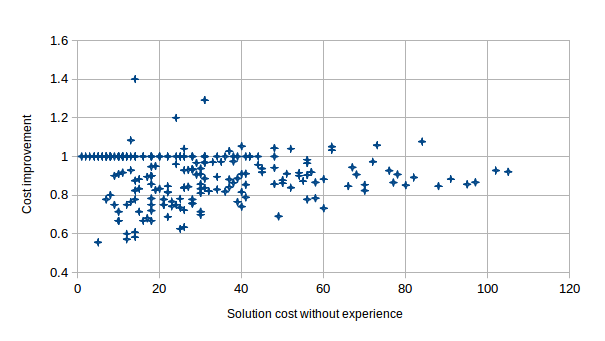
\includegraphics[scale=0.5]{Cost_100_20.png}
	\caption{Relative plan costs using 100\% of the control experience, displaced 20 steps from the control query.}
	 \label{fig:c_100_20}
\end{figure}


\begin{table}
	\centering
	\resizebox{\columnwidth}{!}{%
	    \begin{tabular}{| r | c | c | c | c |}
	    \hline
	    Domain & Inst & 5 steps & 20 steps & 50 steps
	    \\ \hline
	    blocks & 35 & 2.12-7.92 & 2.12-8.70 & 2.21-6.25
	    \\ 
	    driverlog & 14 & 0.86-2.42 & 0.85-1.30 & 0.82-1.20
	    \\ 
	    elevators & 30 & 1.09-4.04 & 0.99-2.76 & 0.90-2.06
	    \\ 
	    grid & 2 & 2.21-3.71 & 1.11-1.34 & 1.10-1.30
	    \\ 
	    logistics00 & 28 & 1.00-1.15 & 0.90-1.11 & 0.84-1.18
	    \\ 
	    logistics98 & 5 & 1.01-2.95 & 0.82-2.06 & 0.80-2.41
	    \\ 
	    pipesworld-notankage & 15 & 1.09-5.30 & 1.00-5.46 & 1.00-2.88
	    \\ 
	    pipesworld-tankage & 8 & 1.00-1.20 & 0.99-1.00 & 1.00-1.13
	    \\ 
	    rovers & 13 & 1.00-1.50 & 1.00-1.00 & 1.00-1.00
	    \\ 
	    satellite & 16 & 0.91-1.25 & 0.87-1.15 & 0.90-1.43
	    \\ 
	    scananalyzer & 16 & 0.74-1.52 & 1.00-1.00 & 1.00-1.00
	    \\ 
	    transport & 23 & 1.26-1.91 & 0.93-1.87 & 0.98-1.46
	    \\ 
	    zenotravel & 13 & 0.80-1.27 & 0.84-1.02 & 1.00-1.00
	    \\ \hline
	    TOTAL & 218 & 0.99-2.72 & 1.00-2.07 & 1.00-1.88
	    \\ \hline
	    \end{tabular}%
	}
	\caption{Experiment 2 speedup statistics, summarized in the form (1st quartile)-(3rd quartile).}
	 \label{tab:walk}
\end{table}

\section{Discussion}

Figures \ref{fig:s_20_0} to \ref{fig:s_100_50} display the individual speedups achieved over all of our experimental trials. We observe that cases in which E-Graphs mislead the planner into generating more states (i.e. speedup $<$ 1) are quite rare, so it seems experiences can only help. We set the bias parameters arbitrarily; tuning them by domain or problem size may well yield even better results. Interestingly, we observe a clear positive correlation between problem size or difficulty, as measured by the number of nodes generated in the control, and the speedup factor. This suggests E-graphs may be especially helpful on the hardest problems.

On the other hand, there is some overhead to E-Graph usage.
Although we explained in the theoretical analysis that the overhead is not too large, constant factors do matter in practice, particularly when the speedups are still in the single-digits.
We measured the number of nodes generated instead of the time taken to complete each search, so as to produce deterministic results which are independent of most engineering details.
Our experiments serve as a proof-of-concept for our approach.

However, some additional work remains before state-of-the-art performance can be achieved.
Aside from engineering optimizations and integration with newer state-of-the-art heuristics, future work will need to consider more intelligent ways to generalize from the experiences encoded by E-Graphs.
This presents a unique challenge in symbolic planning, as distinct states, even if separated by a large distance in the state transition graph, may still be conceptually related.
Thus, a planner could potentially benefit by learning to transfer experiences between parts of the state space which are somehow related.
With such an approach, it would be essential to limit overgeneralization, so as not to waste too much time on false leads.

Finally, we remark that the Experience-Biased HSP algorithm is highly parallelizable, even if A* is retricted to expanding nodes sequentially. Recall that the sum, min and max functions are computable in logarithmic time using linearly many processors. Therefore, with minor adjustments, ComputeG($S$) has parallel depth $O(\mathbf{A\log A\log O})$. With $\mathbf{A\max(O,V^E)}$ processors, the total cost of generating a state is $O(\mathbf{(A\log O + \log V^E)\log A})$. Using even more processors, the cost of \textit{expanding} a state can be reduced to the same by generating its successors in parallel. If still more processors are available, some may be dedicated to the task of preemptively computing $h^E$ for states that are likely to be generated in the future, e.g. near the E-graph or A* frontier.

\begin{figure}
	\centering
	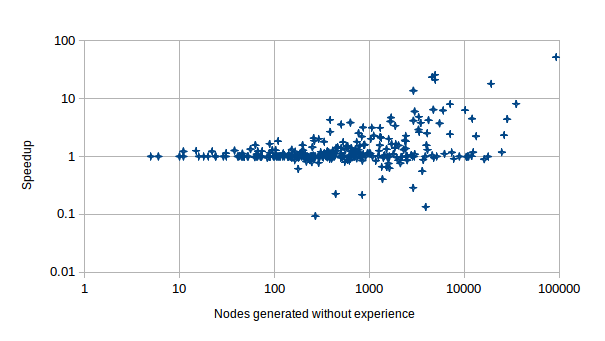
\includegraphics[scale=0.5]{Speedup_20_0.png}
	\caption{Speedups when planning with 20\% of the control experience, displaced 0 steps from the control query.}
	 \label{fig:s_20_0}
\end{figure}

\begin{figure}
	\centering
	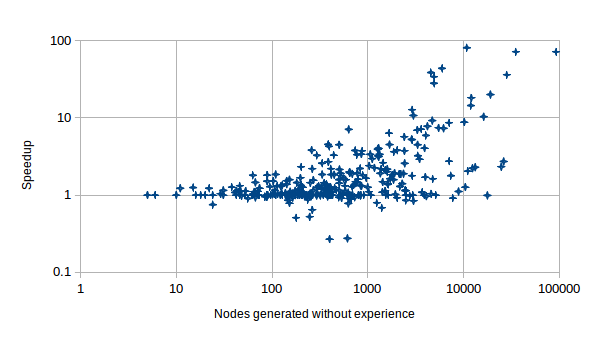
\includegraphics[scale=0.5]{Speedup_50_0.png}
	\caption{Speedups when planning with 50\% of the control experience, displaced 0 steps from the control query.}
	 \label{fig:s_50_0}
\end{figure}

\begin{figure}
	\centering
	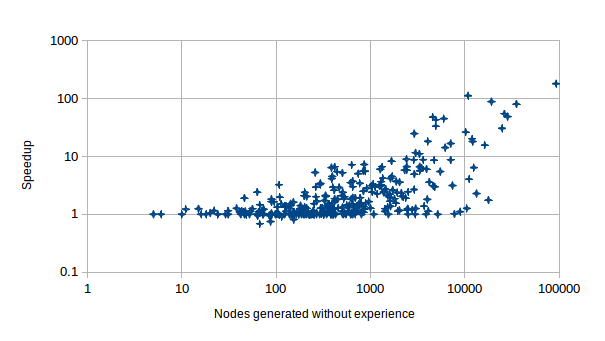
\includegraphics[scale=0.5]{Speedup_80_0.png}
	\caption{Speedups when planning with 80\% of the control experience, displaced 0 steps from the control query.}
	 \label{fig:s_80_0}
\end{figure}

\begin{figure}
	\centering
	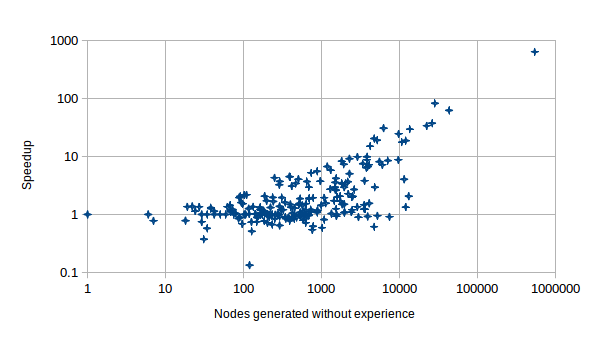
\includegraphics[scale=0.5]{Speedup_100_5.png}
	\caption{Speedups when planning with 100\% of the control experience, displaced 5 steps from the control query.}
	 \label{fig:s_100_5}
\end{figure}

\begin{figure}
	\centering
	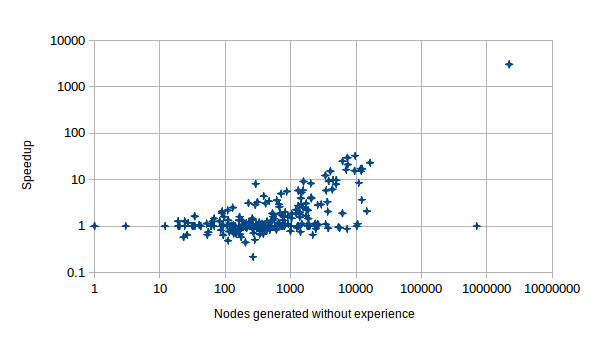
\includegraphics[scale=0.5]{Speedup_100_20.png}
	\caption{Speedups when planning with 100\% of the control experience, displaced 20 steps from the control query.}
	 \label{fig:s_100_20}
\end{figure}

\begin{figure}
	\centering
	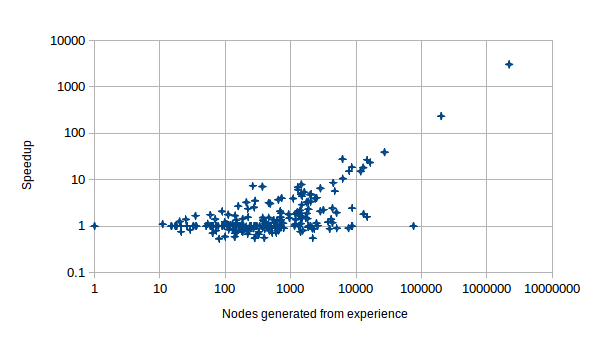
\includegraphics[scale=0.5]{Speedup_100_50.png}
	\caption{Speedups when planning with 100\% of the control experience, displaced 50 steps from the control query.}
	 \label{fig:s_100_50}
\end{figure}

\section{Conclusions}

We saw that, by reusing pieces from past plans, E-Graph-based planners can find solutions more quickly as they learn and acquire experiences. Many interesting directions remain for future investigation. It remains unclear how the bias parameters should be set. In addition, more advanced schemes will be needed to expand and prune E-Graphs if they grow large from collecting a lot of solutions. Keeping track of the most recently computed plans seems like a good idea intuitively, but other possibilities may be worth trying.

As mentioned in the discussion, generalization and parallelization certainly merit further investigation. Generalization is a particularly important problem in AI learning theory, and there is plenty of literature on the topic. For example, \cite{fikes1972learning} generalize plans on the original STRIPS problem solver. The problem of generalization seems related to that of abstraction, or automatically extracting structural information from a symbolic domain or problem description. Works such as \cite{helmert2007flexible} project symbolic state graphs onto smaller spaces; one could potentially apply E-graphs on the projected space to achieve the desired generalization.

E-Graphs should be thought of not so much as a specific algorithm, but as a tool which is orthogonal to a lot of the major planning techniques out there. In principle, one could apply E-Graphs to any of the state-of-the-art A* heuristic-based planners, and one might even adapt the method to obtain anytime, incremental search using experiences as in \cite{phillips2013anytime}, but in symbolic domains.

Finally, E-Graphs might find other uses, such as in replanning. If an unexpected event invalidates a robot's plan mid-execution, the replanner can recall the original solution as an E-Graph to encourage reparations along the old path. In addition to speeding up replanning, the E-Graph could result in a less disruptive solution, in the sense that it avoids unnecessarily deviating from the original plan. Minimizing disruption is important when resources must be allocated in advance according to the plan, or when cognitively-burdened humans are involved with its execution.

\bibliographystyle{aaai}
\bibliography{paper}

\end{document}
